\documentclass[11pt]{article}
\usepackage{graphicx}
\usepackage{amsmath}

\begin{document}

\title{SPS Coursework 2 Report}
\author{Michael Mafeni and Ainesh Sevellaraja}
\date{}
\maketitle

\section{Feature Selection}
We first plotted a 13x13 scatter plot for all pairwise combinations of features of the training data set, as seen below.

%in Figure \ref{fig:13x13}.

%\begin{figure}
%\centering
\begin{center}
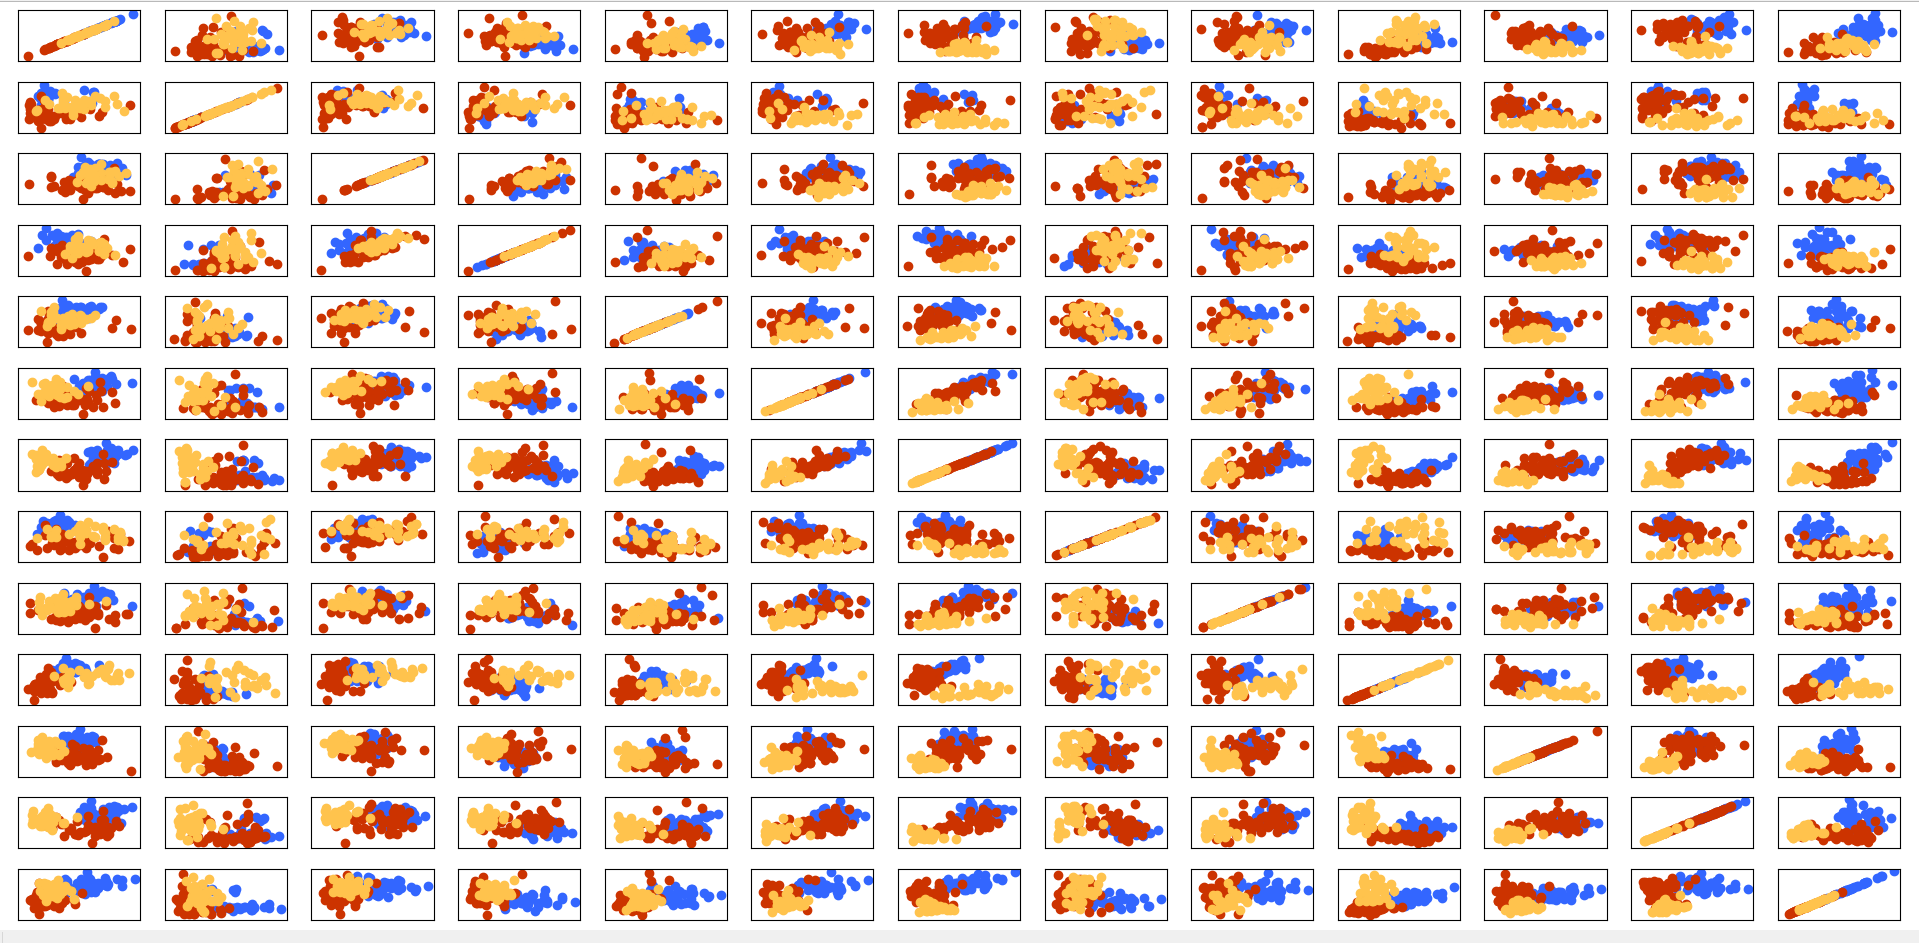
\includegraphics[scale=0.25]{feature_selection}
\end{center}
%\caption{13x13 plot of pairwise combinations of features}
%\label{fig:13x13}
%\end{figure}

Based on the plot above, we decided to select features 10 and 12 as the data separate into their classes fairly well. We then reduced the train set and test set to only contain features 10 and 12. We chose these features as they separted the data into their vatious classes really well. However, this choice was very hard to make from the scatter plot as many plots looked very similar.This can be seen in the scatter plot can be seen below.
% in Figure \ref{fig:10and12}.

%\begin{figure}
%\centering
\begin{center}
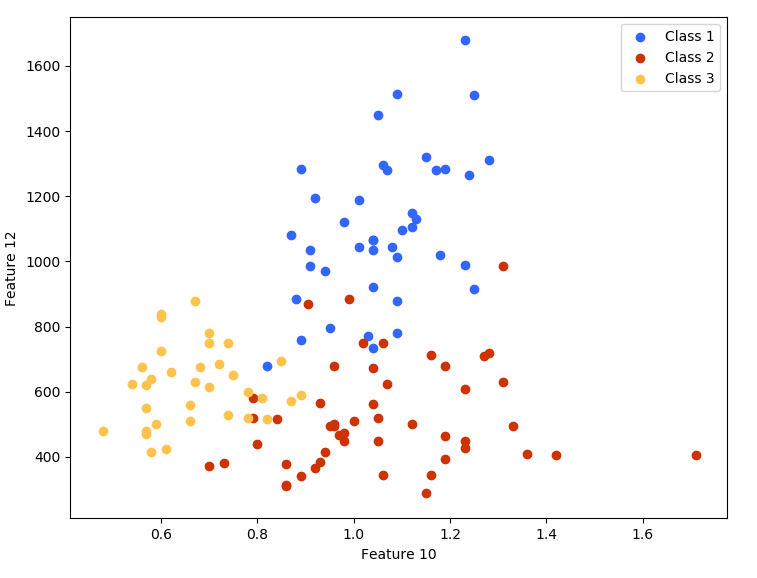
\includegraphics[scale=0.3]{features_10_12}
\end{center}
%\caption{Features 10 and 12 isolated}
%\label{fig:10and12}
%\end{figure}

\section{K-Nearest Neighbours (KNN)}
We implemented the K-Nearest Neighbours classifier. By setting $k = \{1,2,3,4,5,7\}$ our classifier gave the following accuracies and confusion matrices when run with the reduced test set.

%\begin{table}
\begin{center}
\begin{tabular}{c|c|c}
\textbf{k} & \textbf{Accuracy}\\
\hline
1 & 0.7925\\
2 & 0.6792\\
3 & 0.7358\\
4 & 0.7358\\
5 & 0.6981\\
7 & 0.7358\\
\end{tabular}
\end{center}
%\end{table}

\begin{center}
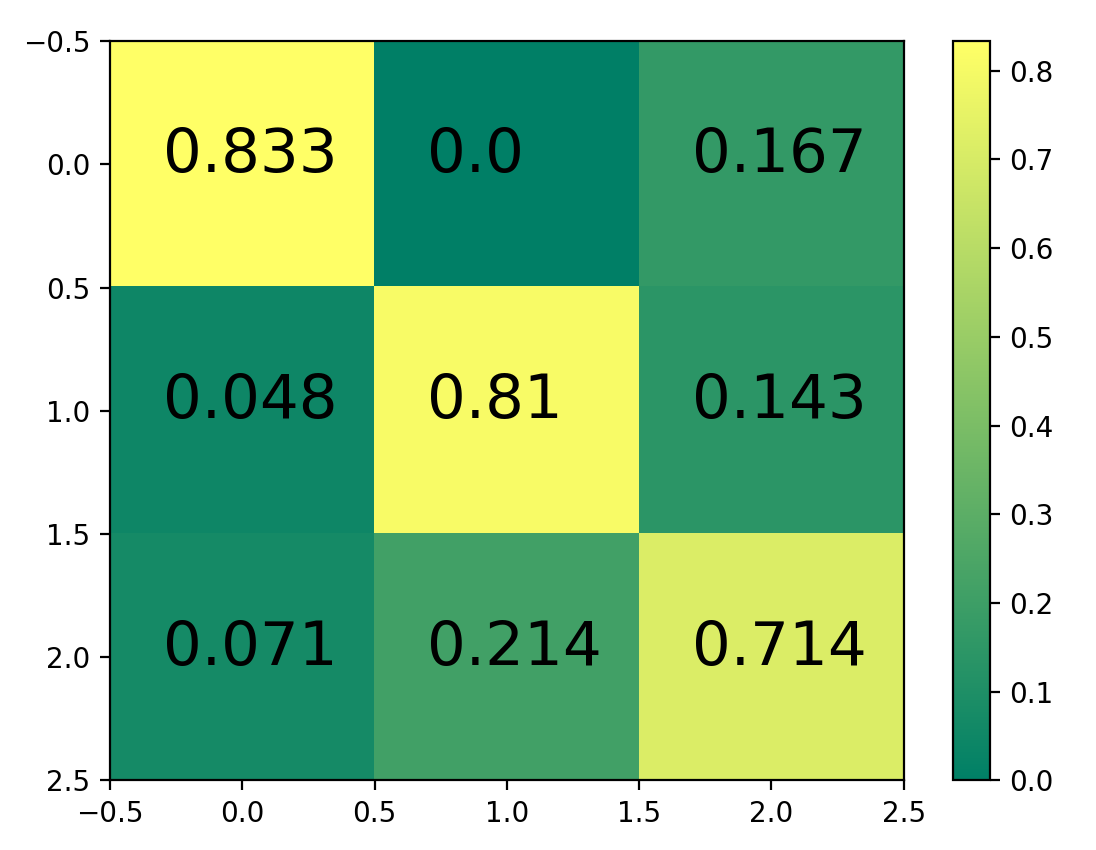
\includegraphics[scale=0.2]{Confusion_matrix(k=1)}
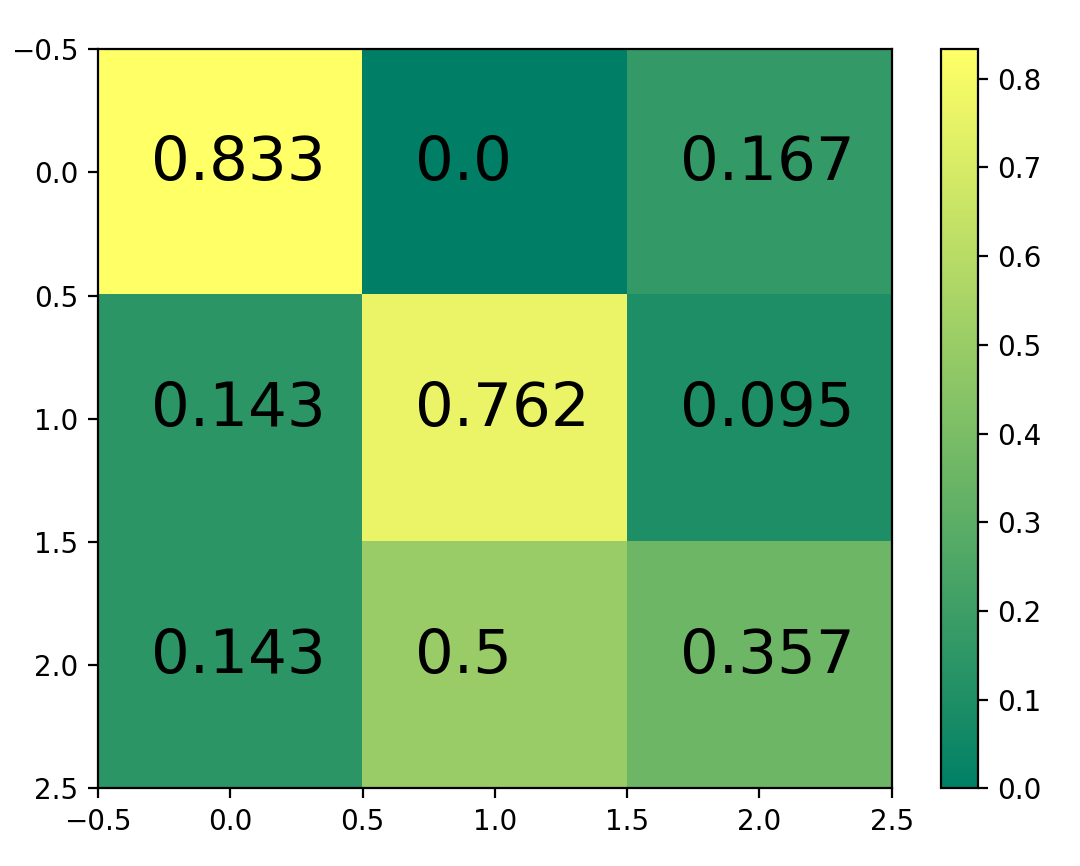
\includegraphics[scale=0.2]{Confusion_matrix(k=2)}
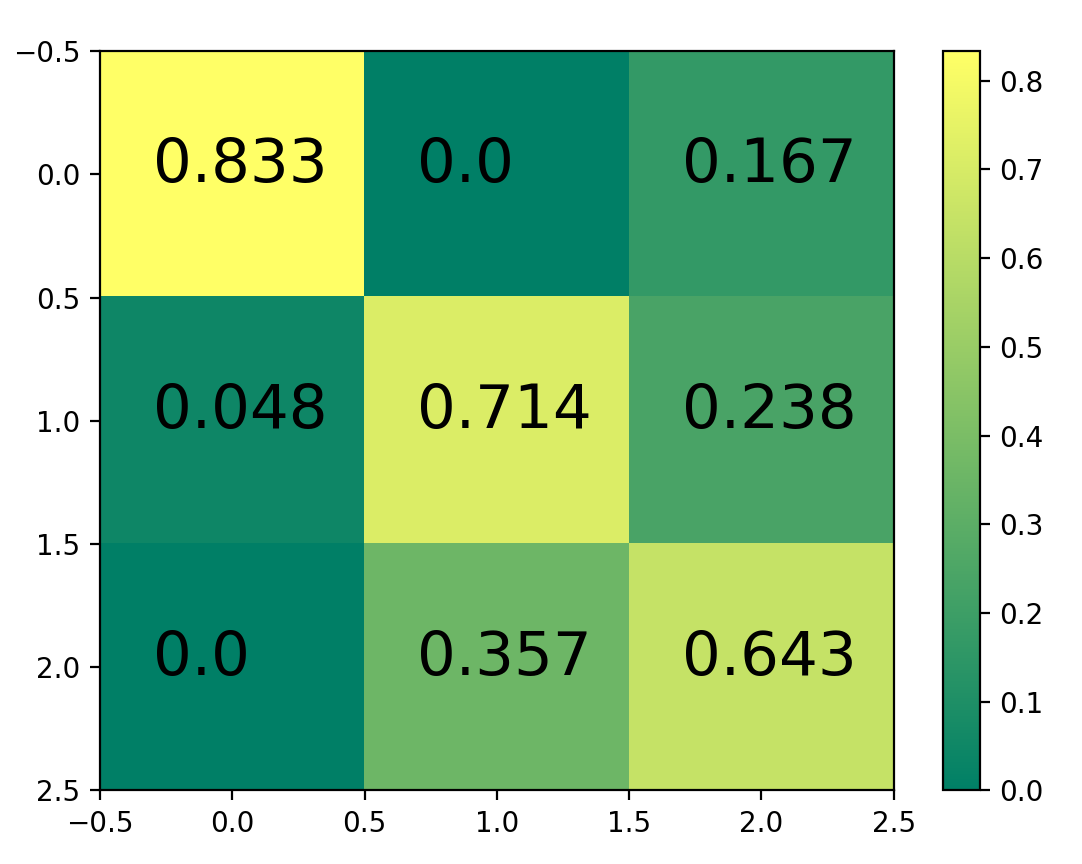
\includegraphics[scale=0.2]{Confusion_matrix(k=3)}
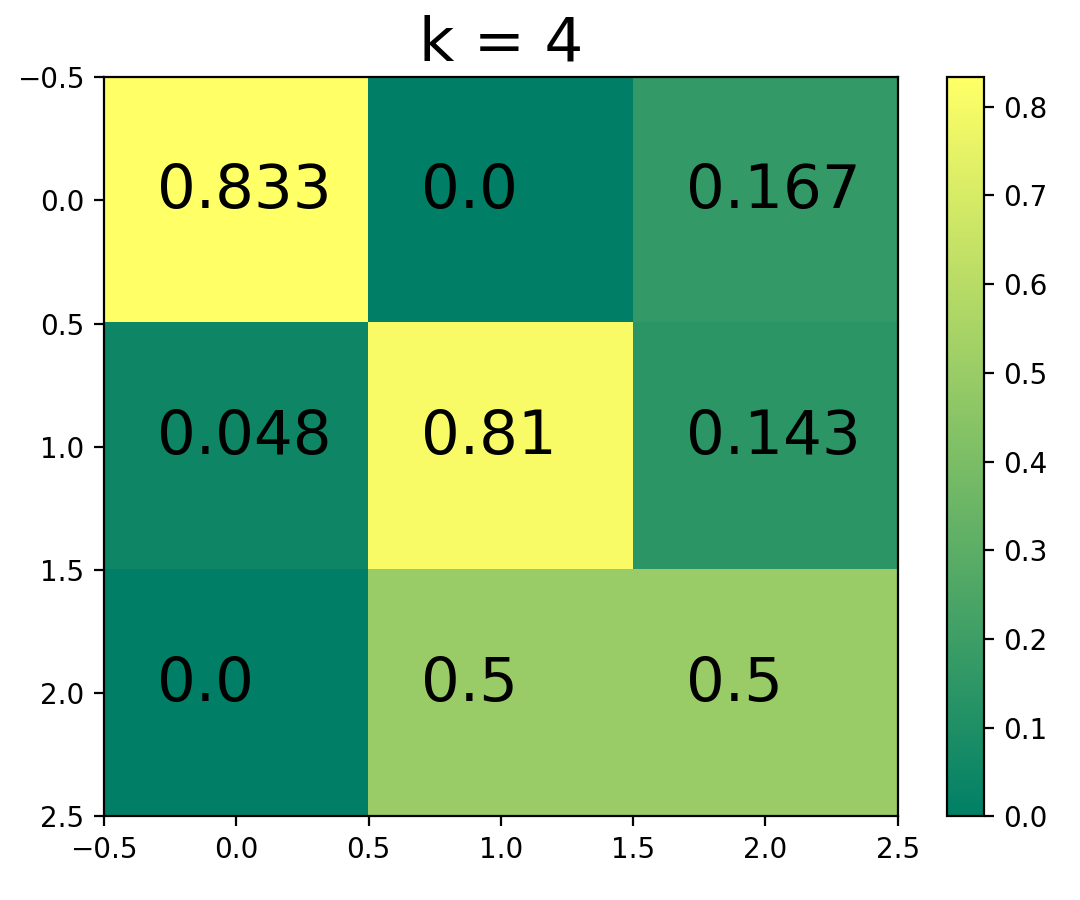
\includegraphics[scale=0.2]{Confusion_matrix(k=4)}
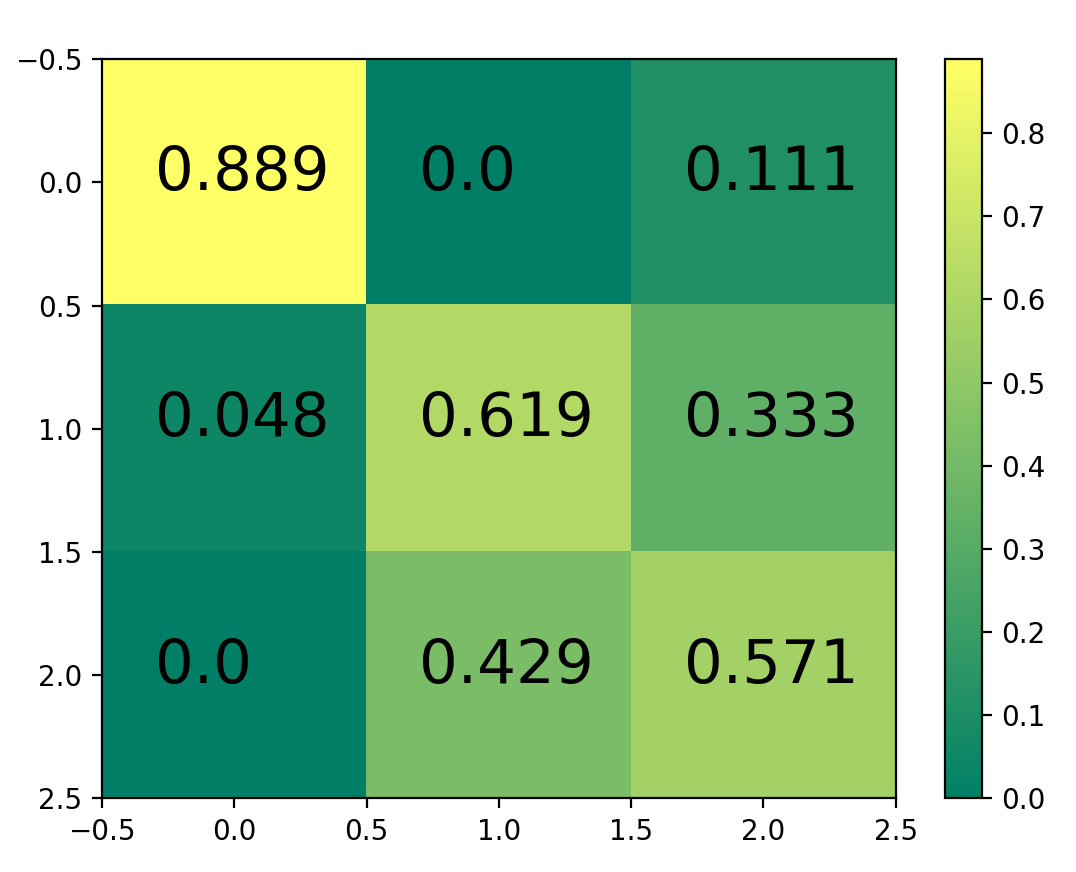
\includegraphics[scale=0.2]{Confusion_matrix(k=5)}
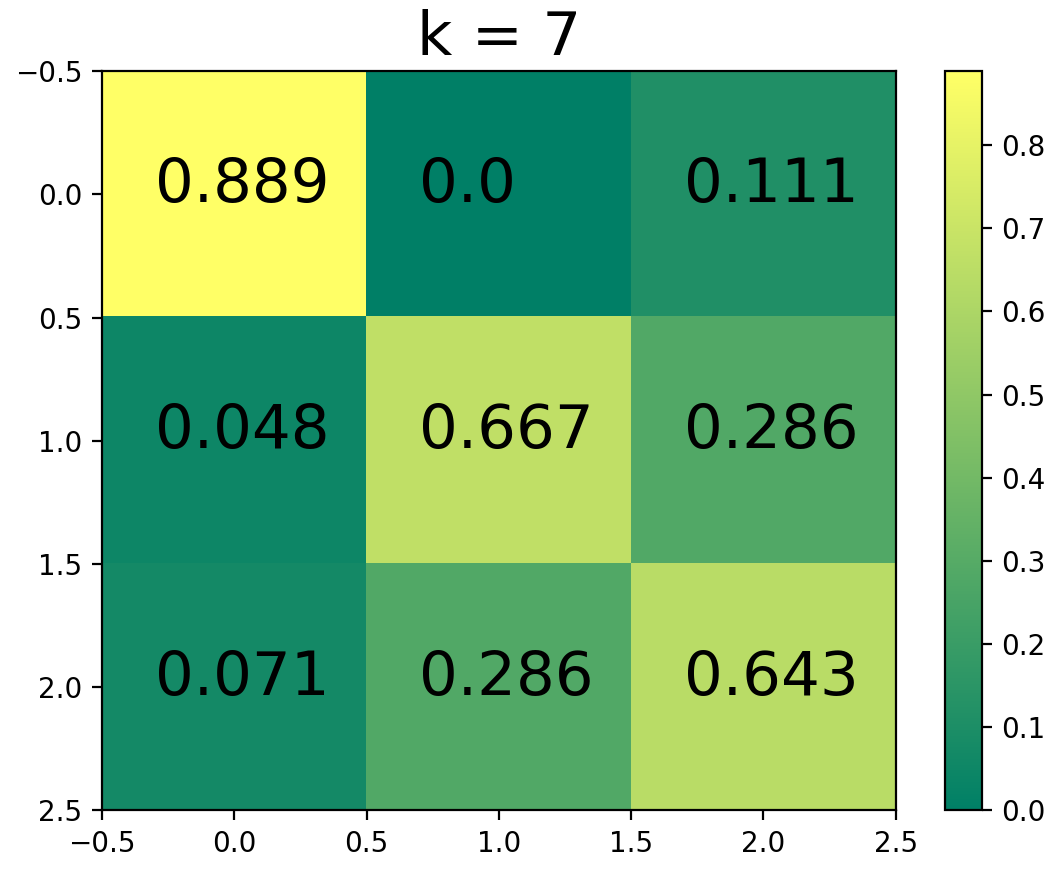
\includegraphics[scale=0.2]{Confusion_matrix(k=7)}
\end{center}

As seen in the table, our classifier gives the highest accuracy when $k = 1$. According to the confusion matrices, a larger portion of test samples in class 1 are correctly classified as $k$ increases. Classes 2 and 3 on the other hand have fewer correctly-classified predictions as k increases. As $k$ increases, a higher portion of test samples in class 3 are incorrectly-classified in class 2, especially when $k = 2$. This may also be a reason why our classifier gives the lowest accuracy when $k = 2$.

The confusion matrices tell us that class 1 has the most data samples correctly predicted. This can also be seen in our scatter plot of feature 12 against feature 10 above, where the blue class which represents class 1 is visibly separated from the other two classes, which leads to a lower chance of class 1 being misclassified.

\section{Alternative Classifier}
For our alternative classifier, we have implemented the Naive Bayes classifier. We assumed the features selected to be independent and normally distributed. This classifier gives an accuracy of 0.8679, which is higher than that our KNN classifier. The classifier gives the following confusion matrix.

\begin{center}
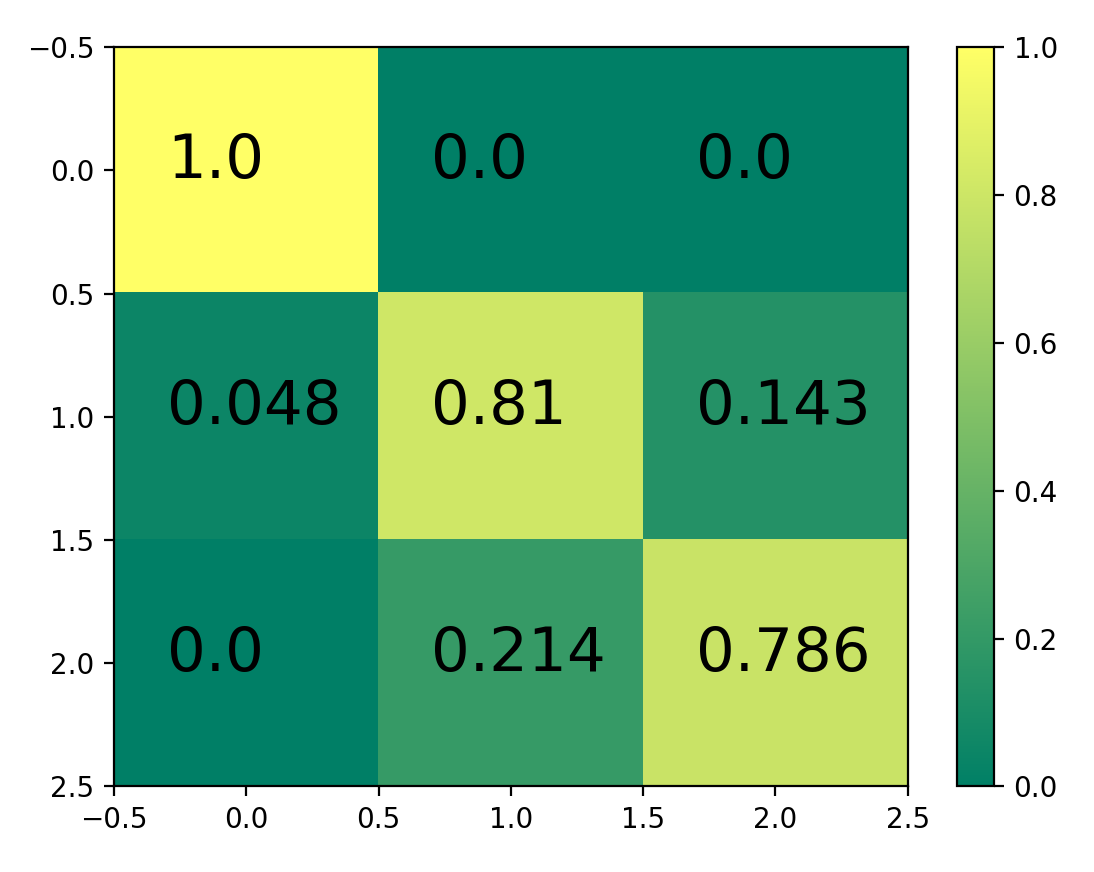
\includegraphics[scale=0.2]{naive_bayes_matrix}
\end{center}

The confusion matrix tells us that all test data samples in class 1 were correctly classified. Hence, our assumption of the features being independent was reasonable for this as we obtained a higher accuracy than with KNN. This also strengthens our point of class 1 being more isolated from the other classes. We did not have to worry about smoothing as we assumed the features to be normally distributed, meaning that the probabilities never reach 0.

\section{Use Three Features}
To obtain the third feature for our KNN classifier, we calculated the covariance matrices of the two already-selected features and every other feature. We picked the feature 7 as it least correlates with features 10 and 12, thus telling us somethingnew about our data. The covariance matrix and scatter plot for these features are as follows:

$$
\bordermatrix{ ~ & ~ & ~ & ~ \cr
Feature 10 & 5.26\times10^{-2} & 1.93\times10^1 & -8.47\times10^{-3} \cr
Feature 12 & 1.93\times10^1 & 9.59\times10^4 & -1.35\times10^1 \cr
Feature 7 & -8.47\times10^{-3} & -1.35\times10^1 & 1.53\times10^{-2} \cr}
$$

\begin{center}
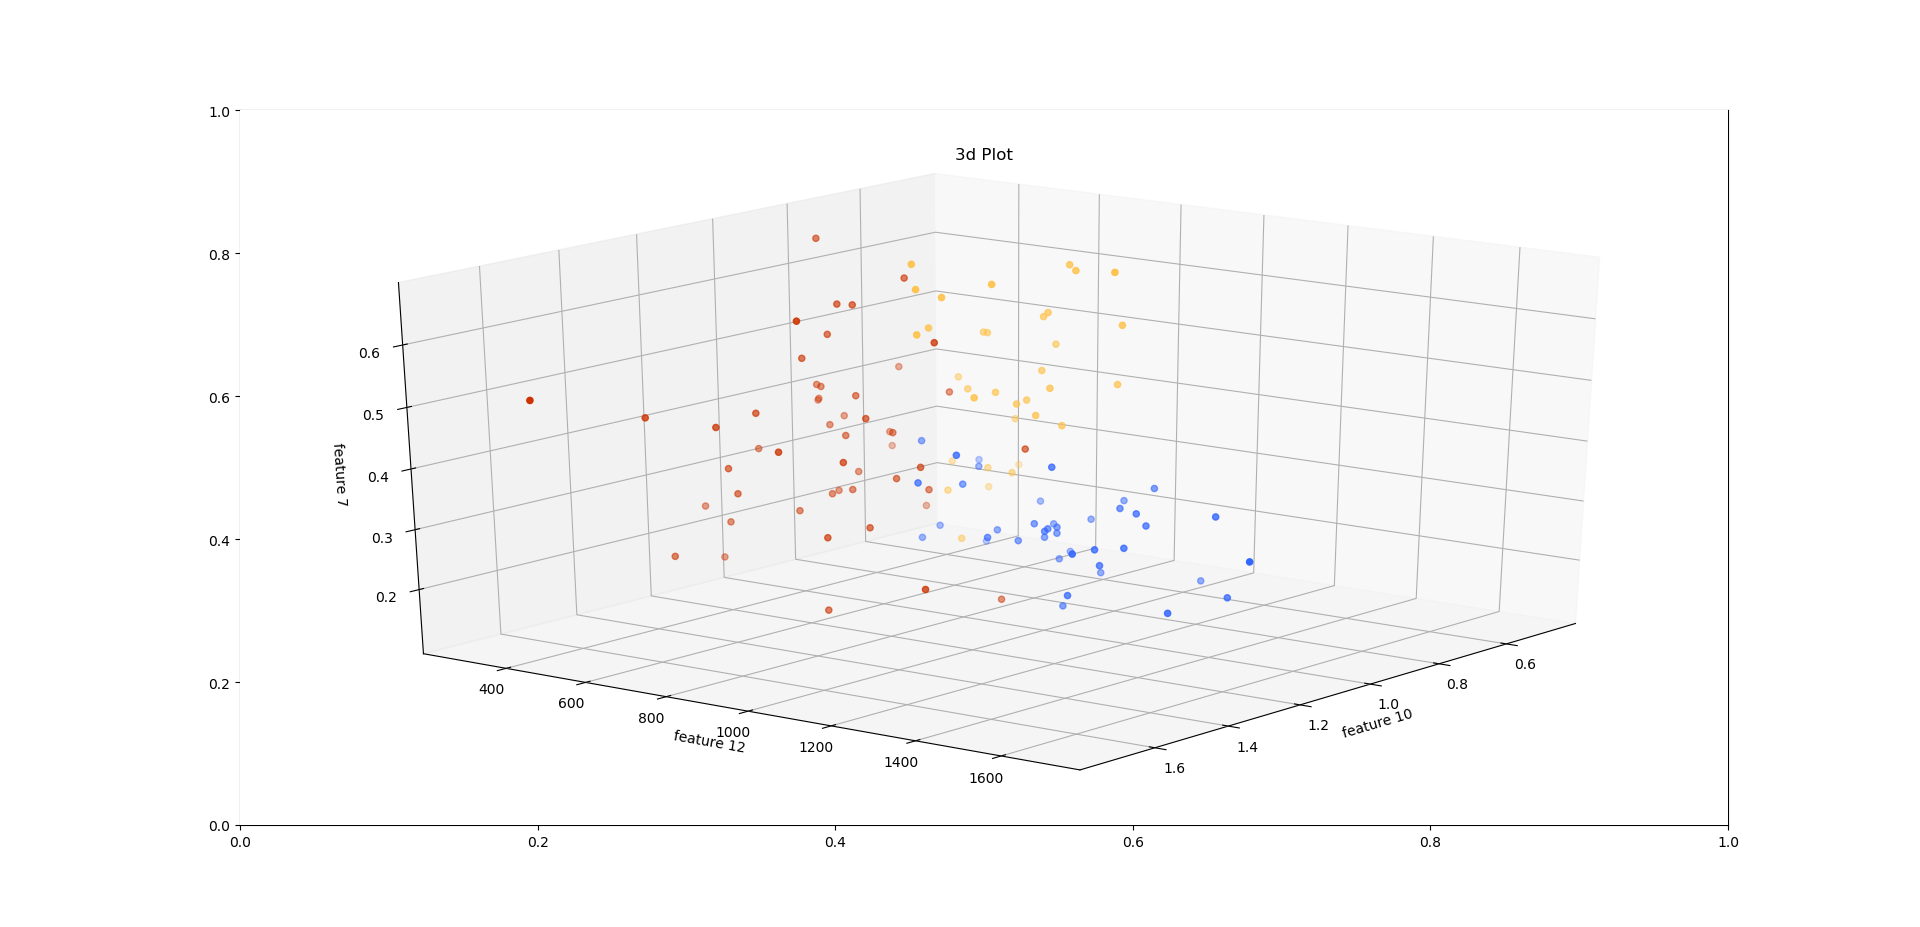
\includegraphics[scale=0.25]{3d_plot}
\end{center}

When KNN is run using these three features at $k = 1$, an accuracy of 0.8302 is achieved which is higher than with two features. This is because adding another feature made our reduced train set more representative of the original train set. However, this made it harder to interpret visually as seen by the 3D scatter plot above.

\section{Principal Component Analysis (PCA)}
We used Scipy's PCA implementation on the train set to reduce it, and obtained the following scatter plot:
\begin{center}
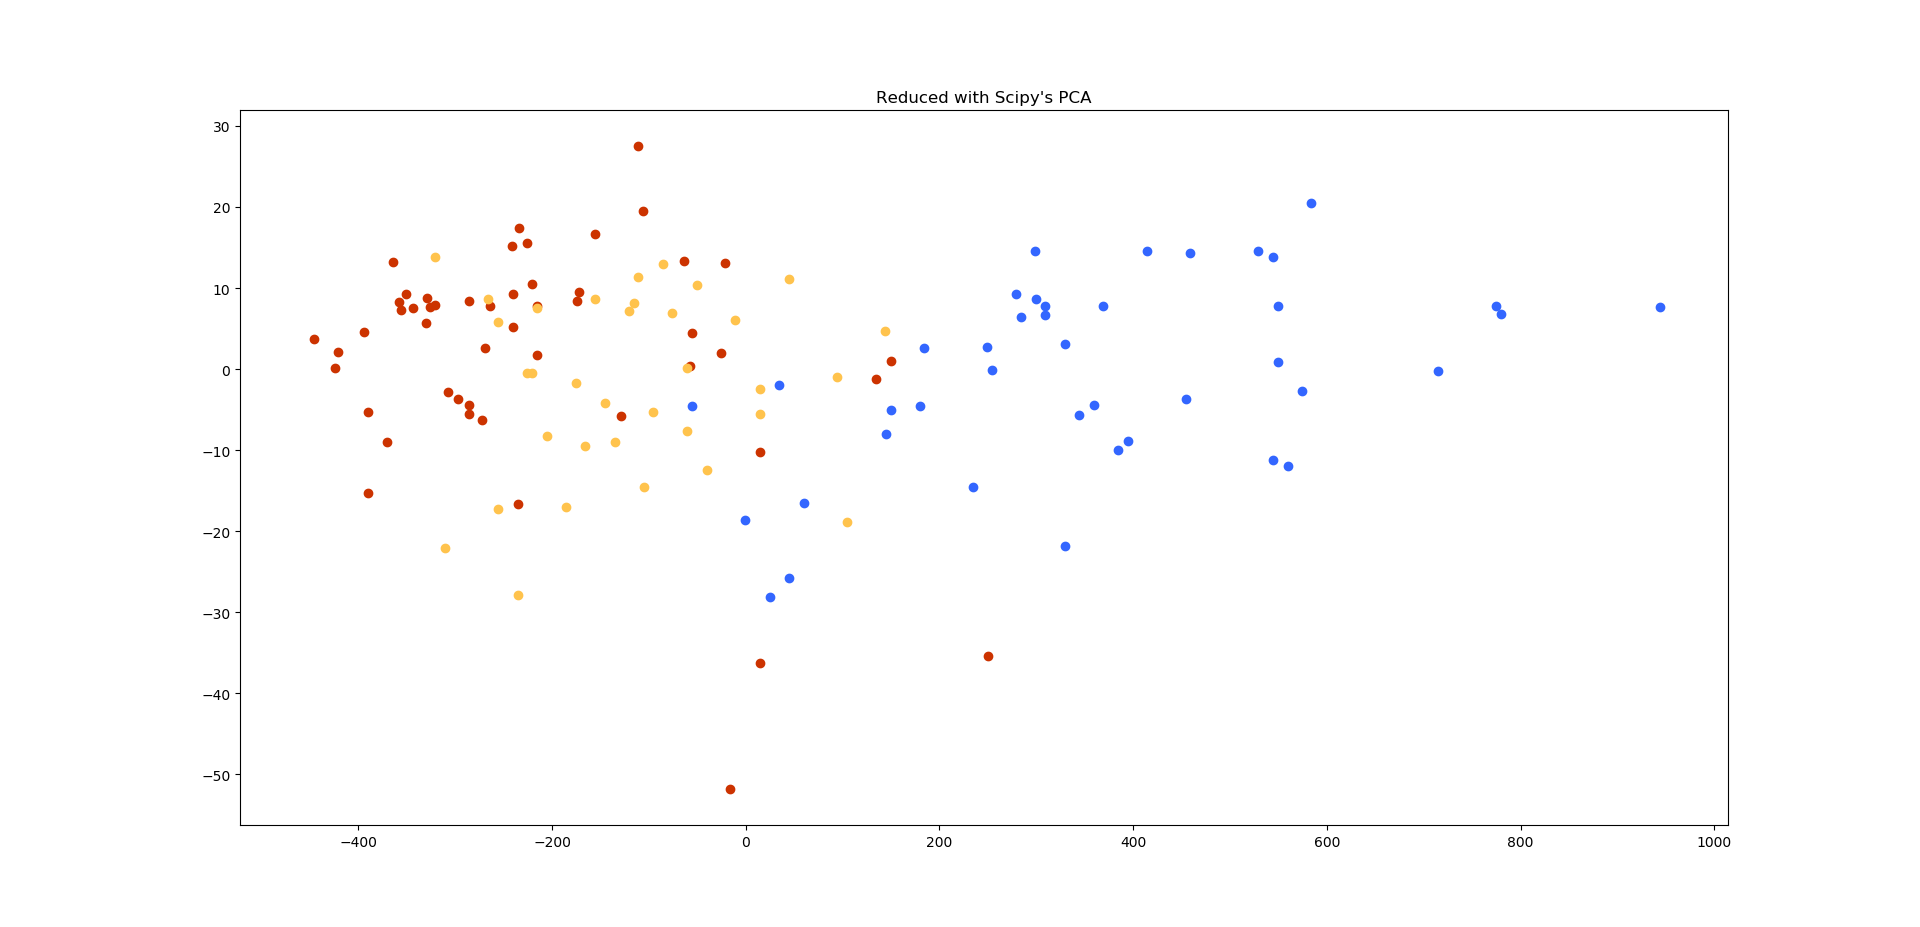
\includegraphics[scale=0.2]{pca_scatter_graph}
\end{center}

After using the model to reduce the test set, we then ran KNN with this reduced train and test set and an accuracy of 0.6792 was obtained when $k = 1$. This is lower than with our manually selected features, which can also be seen via the scatter plot as there is a less distinct boundary between classes 2 and 3 in the PCA plot. This may be because our data only has 13 dimensions, whereas PCA is most effective with higher dimensionality.

\end{document}
